\subsection{Bloch's Equation}
The pulse sequence diagram of an inversion-recovery spin echo sequence is given below.
The sequence is composed of a $\pi_y$ pulse, a $-\frac{\pi}{2}_y$ pulse and a $\pi_x$ pulse and it uses the
following parameters $TE$ = \SI{40}{\milli\s}, $TI$ = \SI{300}{\milli\s} and $TR$ = \SI{1500}{\milli\s}. The sequence is
employed to image a tissue with $T_1$ = \SI{1000}{\milli\s} and $T_2$ = \SI{80}{\milli\s}.
\begin{figure}[h!]
    \centering
    \includegraphics{./homework4/img/pulse_sequence.png}
    \caption{}
    \label{fig:my_label}
\end{figure}




\subsubsection{Consider a spin that precesses with off-resonance frequency equal to 1 Hz. Plot the
evolution of the angle of the transverse magnetization for the above spin for the $\mathbf{2^{nd}}$ $TR$.
Show that the spin echo is formed at time $TE$ from the $\mathbf{-\frac{\pi}{2}_y}$ RF pulse.}

\begin{figure}[h!]
\centering
    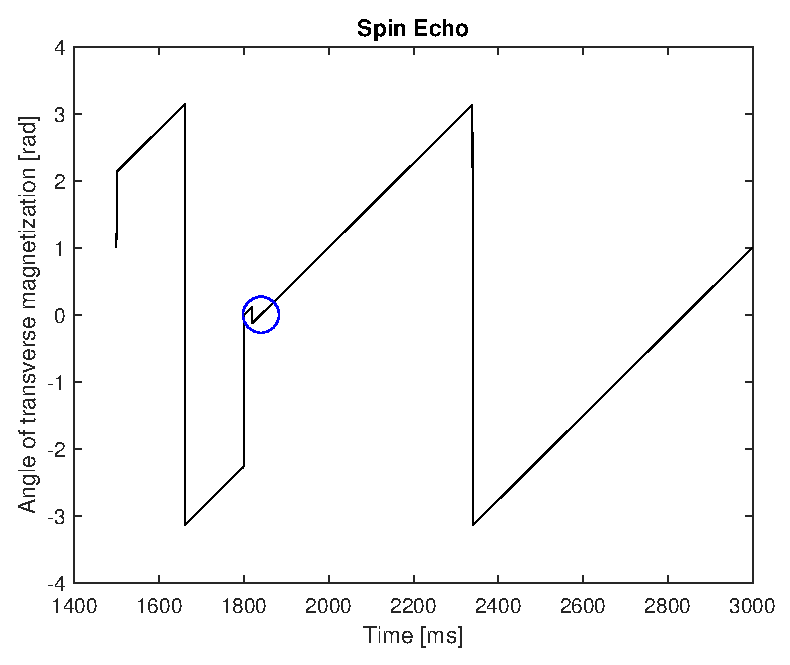
\includegraphics[width=\linewidth]{./homework4/img/Spin_Echo.eps}
    \caption{A spin echo is formed at $T_{echo} = TR\ +\ TI\ +\ TE\ =\ 1840\ ms$ (red circle).}
    \label{fig:spin_echo}
\end{figure}


\begin{lstlisting}
%% Assignment 1:
close all;
clear all;
df = 1; % Hz off-resonance.
T1 = 1000; % ms.
T2 = 80; % ms.
TE = 40; % ms.
TR = 1500; % ms.
TI = 300; % ms.
flip1 = pi; % pi y pulse
flip2 = -pi/2;% -pi/2 y pulse
flip3 = pi; % pi x pulse
dT = 1;
N_tr = round(TR/dT);
N_ti = round(TI/dT);
N_te = round(TE/dT);
N_tehalf = round(TE/(2*dT));
N_ex = 5; % number of RF excitations.
% magnetization vector
M=zeros(3,N_ex*N_tr);
% initial magnetization
M(:,1) = [0;0;1];
% Bloch equation matrices
R_flip1 = yrot(flip1);
R_flip2 = yrot(flip2);
R_flip3 = xrot(flip3);
[A1,B1] = freeprecess(dT,T1,T2,df);
% simulate Bloch equations
M_count=1;
% simulate Nex TRs
for n=1:N_ex
% pi RF excitation
M(:,M_count) = R_flip1*M(:,M_count);
% free-precession and relaxation over period TI
for k=1:N_ti
M_count=M_count+1;
M(:,M_count)=A1*M(:,M_count-1)+B1;
end
% pi/2 RF excitation
M(:,M_count) = R_flip2*M(:,M_count);
% free-precession and relaxation over period TR-TI
for k=1:N_tehalf
M_count=M_count+1;
M(:,M_count)=A1*M(:,M_count-1)+B1;
end
% pi RF excitation
M(:,M_count) = R_flip3*M(:,M_count);
% free-precession and relaxation over period TR-TI-TE/2
for k=1:(N_tr-N_ti-N_tehalf)

M_count=M_count+1;
M(:,M_count)=A1*M(:,M_count-1)+B1;
end
end
time = [0:M_count-1]*dT;
%% verify formation of echo by plotting angle of transverse magnetization
% for second TR
M_trans=M(1,:)+j*M(2,:);
figure;
plot(time(N_tr:2*N_tr),angle(M_trans(N_tr:2*N_tr)),'k-');
hold on;
scatter(N_tr+TI+TE,angle(M_trans(N_tr+TI+TE+1)), 300, 'b');
xlabel('Time [ms]');
ylabel('Angle of transverse magnetization [rad]');
title('Spin Echo');
print('img/Spin_Echo.eps','-depsc');
\end{lstlisting}

\subsubsection{Plot the evolution of longitudinal and transverse magnetization for 5 TRs. How many
TRs are required in order to establish a steady-state in the magnetization evolution?}
The stead state in the magnetization evolution is reached after $2\ TR$. (Fig. \ref{fig:inv_rec})
\begin{figure}[h!]
\centering
    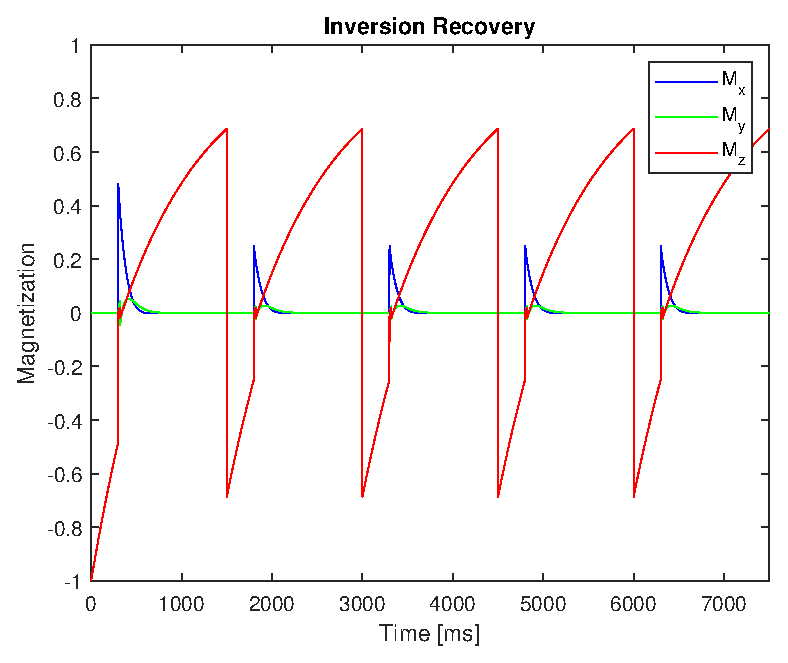
\includegraphics[width=\linewidth]{./homework4/img/Inversion_Recovery.eps}
    \caption{Inversion Recovery splitted into trajectories of the three cartesian field components.}
    \label{fig:inv_rec}
\end{figure}



\begin{lstlisting}
%% plot magnetization evolution
figure;
time = [0:M_count-1]*dT;
plot(time,M(1,:),'b-',time,M(2,:),'g-',time,M(3,:),'r-');
legend('M_x','M_y','M_z');
xlabel('Time [ms]');
ylabel('Magnetization');
axis([min(time) max(time) -1 1]);
title('Inversion Recovery');
print('img/Inversion_Recovery.eps','-depsc');
\end{lstlisting}


\subsubsection{Based on the numerical simulation of the Bloch equation, determine the signal of the
spin echo at the $\mathbf{5^{th}}$ TR (assume $\mathbf{M_0=1}$). Compare the signal of the formed spin-echo at the
$\mathbf{5^{th}}$ TR to the following analytical expression (depending on $\mathbf{T_1}$ and $\mathbf{T_2}$ relaxation times):}
The error between simulated and analytical solution is in the $3^{rd}$ digit. Hence, the simulation shows an accurate approximation.
\begin{align}
S\ &=\ M_0\left( 1-2e^{-\frac{TI}{T_1}}\ +\ 2e^{-\frac{TR-\frac{TE}{2}}{T_1}}\ -\ e^{-\frac{TR}{T_1}}\right)\ \cdot\ e^{-\frac{TE}{T_2}}\\
M_{echo,\ 5^{th}TR_x}\ &=\ 0.1532\\
M_{analytical,\ x}\ &=\ 0.1568
\end{align}

\begin{lstlisting}
%% signal at TE of the 5th TR based on numerical Bloch equation simulation
M_echo_5thTR = abs(M(:,4*N_tr+ N_ti + N_te));
M_echo_5thTR_x = M_echo_5thTR(1, :)
% signal based on analytical formula
M_analytical_x = abs((exp(-TE/T2))*(1-2*exp(-TI/T1)+exp(-TR/T1)))
\end{lstlisting}

\subsubsection{The above equation can be simplified for $\mathbf{TE<<TR}$:
Based on the analytic above expression, it is possible for a given TR to select the inversion time TI to null the signal of a tissue with a given $\mathbf{T_1}$. Assume that the inversion recovery spin echo sequence will be used to null the signal from fat ($\mathbf{T_1}$=360 ms). Find the inversion time required to null the fat signal.}
\begin{align}
S\ &=\ M_0\left( 1-2e^{-\frac{TI}{T_1}}\ +\ 2e^{-\frac{TR-\frac{TE}{2}}{T_1}}\ -\ e^{-\frac{TR}{T_1}}\right)\ \cdot\ e^{-\frac{TE}{T_2}}\\
S\ &\overset{TE<<TR}=\ M_0\ \left(1-2e^{-\frac{TI}{T_1}} + e^{-\frac{TR}{T_1}} \right) e^{-\frac{TE}{T_2}}\\
S\ &\overset{!}=\ 0,\  T_1(fat)\ =\ \SI{360}{\ms}\ \wedge\  TR\ =\ \SI{150}{\ms}\\
TI\ &=\ -T_1\ \mathrm{ln}\left(0.5\ +\ 0.5e^{-\frac{TR}{T_1}}\right)\\
TI\ &=\ -\SI{360}{\ms}\ \cdot\ \mathrm{ln}\left(0.5\ +\ 0.5e^{-\frac{\SI{150}{\ms}}{\SI{360}{\ms}}}\right)\ =\ \SI{243.94}{\ms}\\
TI_{sim}\ &=\ \SI{243.94}{\ms}
\end{align}

\begin{lstlisting}
T1fat=360; %ms
TR=1500; %ms
TI=-T1fat*log(.5+.5*exp(-TR/T1fat))
S=(1-2*exp(-TI/T1fat) + exp(-TR/T1fat))
\end{lstlisting}